\chapter{Coplanar waveguide}
\section{\label{sec:Coplanar Waveguide Design}Coplanar waveguide design}
This section investigates the quality factor, $Q$ of a coplanar waveguide (CPW) resonator up to the maximum Nb film thickness, $d$ of 300 nm. The temperature regime (~4 $K$) of operation results in the loss being dominated by interactions between thermal quasi-particles.      

\subsection{CPW basics}

\noindent The CPW resonator consists of a center conductor surrounded by ground planes fabricated using the method of optical lithography onto a substrate. There are options of different geometries of capacitively coupled CPW resonators as shown in Fig.~\ref{fig:CPWgoppl08}(a). The conductor coupling enables transmission of input and output signals.

\begin{figure}[h]
\centering
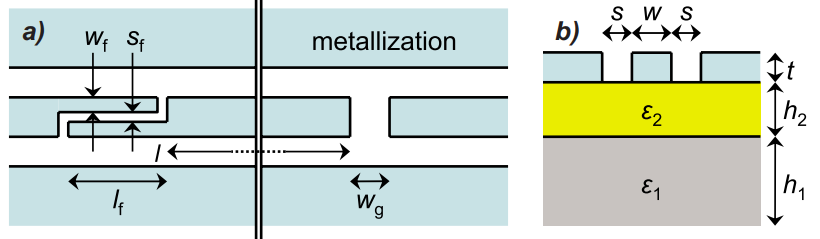
\includegraphics[height=0.3\textwidth,keepaspectratio]{CPWgoppl08}
\caption{\label{fig:CPWgoppl08} (a) CPW top view with finger capacitors (left) and gap capacitors (right). (b) CPW design cross section with a double layer substrate (yellow and grey)~\citep{doi:10.1063/1.3010859}.}
\end{figure}

The CPW cross-sectional view is shown in Fig.~\ref{fig:CPWgoppl08}(b) where the metal thickness is denoted by $t$ is most often referred to in the literature as $d$, therefore I will use the more conventional descriptor $d$. The central conductor width $W$ and the gap between the conductor and ground plane $S$ are values which impact the geometric inductance and capacitance. The capacitance and inductance per unit length are given as:

  

\subsection{CPW Q factor}
The quality factor describes how underdamped (high $Q$) or overdamped (low $Q$) a resonator is. The loaded quality factor is a parallel combination of internal and external (capacitive coupling) quality factors. The model for a LCR resonator quality factor utilised for derivation for the CPW by Yoshida in Ref.~\citep{402973}. The LCR resonator $Q= \frac{\omega L}{R}$ can be derived from considering that $Q$ is ratio of the total energy stored to the total energy lost per cycle\footnote{Useful link: http://www.techlib.com/reference/q.htm}. 

The capacitance and inductance based on the geometry of the CPW are calculated using conformal mapping techniques 


\begin{equation}
\label{eq:quasilimited1}
C_{g}=4\epsilon_{0}\epsilon_{eff}\frac{K(k_{0})}{K_{ko'}}
\end{equation}








total inductance is calculated as the sum of the internal resonator inductance $L_{g}$ and the kinetic inductance $L_{k}$ which are given as: 




The aim is to achieve a $Q$ which is quasi-particles limited:

\begin{equation}
\label{eq:Qquasilimited}
Q_{qp} = \frac{\sigma_{2}}{\sigma_{1}} \left ( 1 + \frac{L_{g}}{L_{k}} \right )
\end{equation} 



\noindent This expression is derived from 

\begin{equation}
\label{eq:quasilimited1}
\frac{\omega_{c}}{(L_{k}+L_{L_{g}})}{Rs}
\end{equation}


